%%This is a very basic article template.
%%There is just one section and two subsections.
\documentclass{article}

\input{fs.tex}
%Title of Document
\chead{Analysis III - Summary} 

\begin{document}
\begin{twocolumn} 

\section{Notation \& Classification}

$$f(x_1, x_2, \ldots, x_n, u, u_{x_1}, u_{x_2}, \ldots, u_{x_1x_1}, \ldots) \qquad u_{x_k} = \frac{\partial u}{\partial x_k}$$

\subsection{Well-Posedness}

A problem is called well-posedness, if it satisfies all of the following criteria:
\begin{enumerate}
	\item \textbf{Existence}: The problem has a solution
	\item \textbf{Uniqueness}: There is no more than one solution
	\item \textbf{Stability}: A small change in the equation or in the side conditions gives rise to a small change in the solution
\end{enumerate}

\subsection{Classification}

\begin{itemize}
	\item \textbf{Order}: The order of a PDE is the order of the highest derivative in the equation.
	\item \textbf{Linear}: An PDE is called linear if the unknown function $u$ and it's derivatives occur only in a linear relationship. 
	\item \textbf{Semilinear}: A PDE is called semilinear if only the unknown function $u$ occurs in a non-linear relationship, but all the partial derivatives of $u$ occur linear.
	\item \textbf{Quasilinear}: A PDE is called quasilinear if the highest order derivative occurs linear in $F$, but lower order derivatives of $u$ and $u$ itself occur non-linear.
\end{itemize}

\subsection{Strong vs. Weak Solutions}

The Set $C^k(D)$ contains all functions that are $k$-times differential in $D$. 
A Function in the Set $C^k(D)$, that satisfies a PDE of order $k$ is called a \textbf{strong} (or \textbf{classical}) \textbf{solution}. 
If the solution is not $k$ times differential, it is called a \textbf{weak solution}.

\subsection{Differential Operators}

The operation of an operator $L$ on a function $u$ is denoted by $L[u]$
A differential Operator is defined by partial derivatives of functions. 
Example:

$$\text{Laplace Operator:} \quad \Delta = \left[\sum_{i=1}^{n} \frac{\partial^2}{\partial x_i^2}\right]$$

A \textbf{linear operator} satisfies the following equation:

$$L[\alpha_1 u_1 + \alpha_2 u_2] = \alpha_1 L[u_1] + \alpha_2 L[u_2]$$

\subsection{Initial Conditions}

A problem is called an \textbf{initial value problem} if a condition at $t = t_0$ is given. Example of the heat equation:

$$u_t - \Delta u = 0 \qquad u(t=0, x, y, z) = u_0$$

\subsection{Boundary Conditions}

Boundary conditions are conditions on the behavior of the solution (or it's derivatives) at the boundary $\partial \Omega$ of the domain $\Omega$. 

\begin{itemize}
	\item \textbf{Dirichlet condition}: In this condition, the values at the boundary $\partial \Omega$ are given (e.g. by measurements)
	
	$$u(x,y,z,t) = f(x,y,z,t) \qquad (x,y,z) \in \partial \Omega, \, t > 0$$
	
	\item \textbf{Neumann condition}: Here, the normal derivative $\partial_n u$ of the unknown function $u$. $\partial_n u$ denotes the outward normal derivative at $\partial \Omega$
	
	$$\partial_n u(x,y,z,t) = f(x,y,z,t) \qquad (x,y,z) \in \partial \Omega, \, t > 0$$
	
	\item \textbf{A condition of a third kind} is a combination of the two mentioned above (sometimes also called a Robin condition).
	
\end{itemize}

\section{First-Order PDE}

$$F(x_1,x_2,\ldots, x_n, u, u_{x_1}, u_{x_2}, \ldots u_{x_n}) = 0$$

\subsection{Method of characteristics}
Solve the following initial value problem (of order 2):

$$a(x,y,u) u_x + b(x,y,u) u_y = c(x,y,u)$$
$$\ex{u_x + u_y = 2u + 1 \quad u(x,0) = 0 \qquad a = 1, \quad b = 1, \quad c = 2}$$

\begin{enumerate}

\item write the characteristic equation and parametric initial condition (for the initial condition, substitute $s$ for $x$ or $y$, depending on the initial condition.)
$$\pdif{x}{t}(t,s) = a(x,y,u) \quad \pdif{y}{t}(t,s) = a(x,y,u) \quad \pdif{u}{t}(t,s) = c(x,y,u)$$
$$\ex{x_t = 1 \quad y_t = 1 \quad u_t = 2u + 1 \qquad x(0,s) = s \qquad y(0,s) = 0 \qquad u(0,s) = 0}$$

\item solve the characteristic equation (by simple integrating or by solving the ODE)
$$\ex{x(s,t) = t + f_1(s), \quad y(s,t) = t + f_2(s), \quad u(s,t) = f_3(s) e^{2t} + t + f_4(s)}$$

Some example of simple ODEs and how to solve them (use superposition):
$$\pdif{x}{t} = \alpha \: \Rightarrow \: x(t,s) = \alpha t + C(s)$$
$$\pdif{x}{t} = \alpha x \: \Rightarrow \: x(t,s) = C(s) e^{\alpha t}$$
$$\pdif{x}{t} = \alpha x + \beta e^{\alpha t} \: \Rightarrow \: x(t,s) = C(s) e^{\alpha t} + \beta e^{\alpha t} \cdot t$$
$$\pdif{x}{t} = \alpha x + \beta e^{\gamma t} \: \Rightarrow \: x(t,s) = C(s) e^{\alpha t} - \frac{\beta e^{\gamma t}}{\alpha - \gamma} \quad \alpha \neq \gamma$$
$$\pdiff{x}{t} = -\alpha x \: \Rightarrow \: x(t,s) = C_1(s) \cos \alpha t + C_2(s) \sin \alpha t$$

\item Substitute these solutions into the initial condition to get $f_i(s)$. If some $f_i(s)$ are undefined, normalize the equation for simplicity.
$$\ex{x(t,s) = t + s \qquad y(t,s) = t \qquad u(t,s) = f(s) e^{2t} + t - f(s), \, f(s) = \frac{1}{2}}$$

\item Solve for $(t,s)$ as a function of $(x,y)$ and write the solution $u$:
$$\ex{t = y, \qquad s = x-y \qquad u(x,y) = \frac{1}{2} e^{2y} + y - \frac{1}{2}}$$
\end{enumerate}


\subsection{Invertibility $(s,t) \;\rightarrow\; (x,y)$ (transversality)}

The relation $(s,t) \; \rightarrow \; (x,y)$ is \textbf{locally} invertable, if and only if:

$$\left. \det \begin{cmatrix}\pdif{x}{t} & \pdif{y}{t} \\ \pdif{x}{s} & \pdif{y}{s}\end{cmatrix} \right|_{x_0,y_0,u_0} = \det \begin{cmatrix}a(x_0,y_0,u_0) & b(x_0,y_0,u_0) \\ \pdif{x_0(s)}{s} & \pdif{y_0(s)}{s} \end{cmatrix} \neq 0$$

\subsection{Existence of a solution}

Sometimes, a calculated solution to the PDE is not valid. 
For this, let $\gamma(s) = (x_0(s),y_0(s),0)$ be the projection of the initial condition to the $(x,y)$-plane. if $(x(s,t_0), y(s,t_0),0) = \gamma(\tilde{s})$ for $t_0 \neq 0$, we must check if the value of the curve equals the value of the initial condition. If $u_0(\tilde{s}) \neq u(s,t_0)$, the solution is not valid.

\textbf{Example:} consider the following PDE:

$$\ex{-y u_x + x u_y  = u \quad u(x,0) = x^2, \qquad x_0(s) = s, \; y_0(s) = 0, \; u_0(s) = s^2}$$
$$\ex{x(s,t) = s \cos t, \quad y(s,t) = s \sin(t), \quad u(s,t) = s^2 e^t}$$

Let $t_0 = \pi$ and $\tilde{s} = -s$. Then:

$$\ex{x(s,t_0)u = x_0(-s), \; y(s,t_0) = y_0(-s), \; u(s,t_0) \neq u_0(-s) \Rightarrow \text{no sol.}} $$ 

\subsection{Conservation laws and shock waves}

Let's consider the following equation, where $y$ is the time.

$$u_y + u u_x = 0, \quad u(x,0) = h(x)$$
$$x(t,s) = s + t \cdot h(s), \quad y(t,s) = t, \quad u(t,s) = h(s) \;\Rightarrow\; u = h(x-uy)$$

The solution is not well defined at points where characteristic curves intersect. From an algebraic perspective:

$$u_x = \frac{h'}{1 + y h'} \qquad y_c = \inf \left\{- \frac{1}{h'(s)} \right\}$$

The classical solution is not defined for $y > y_c$. To extend the solution beyond $y_c$. The solution $u$ has discontinuities at $u(\gamma(y),y)$. $u^-$ and $u^+$ is the value of $u$ when we approach the curve $\gamma$ from the left and from the right, respectively. Then, we get:

$$\gamma(y) = \frac{1}{2} (u^- + u^+)$$

\begin{tabular}{cccc}
	\begin{tikzpicture}[scale=0.7]
		\draw [->] (-1,0) -- (2.5,0) node [above] {\small$x$};
		\draw [->] (0,-0.5) -- (0,1.5) node [left] {\small$u$};
		\draw (1,0) node[below] {\small$\alpha$} (1,-0.08) -- (1,0.08);
		\draw (2.5,1.5) node [left] {\small$y = 0$};
		\draw [thick, cRed] (-1,1) -- (0,1) -- (1,0) -- (2.3,0);
	\end{tikzpicture} &
	\begin{tikzpicture}[scale=0.7]
	\draw [->] (-1,0) -- (2.5,0) node [above] {\small$x$};
	\draw [->] (0,-0.5) -- (0,1.5) node [left] {\small$u$};
	\draw (1,0) node[below] {\small$\alpha$} (1,-0.08) -- (1,0.08);
	\draw (2.5,1.5) node [left] {\small$0 < y < \alpha$};
	\draw [thick, cRed] (-1,1) -- (0.4,1) -- (1,0) -- (2.3,0);
	\end{tikzpicture} &
	\begin{tikzpicture}[scale=0.7]
	\draw [->] (-1,0) -- (2.5,0) node [above] {\small$x$};
	\draw [->] (0,-0.5) -- (0,1.5) node [left] {\small$u$};
	\draw (1,0) node[below] {\small$\alpha$} (1,-0.08) -- (1,0.08);
	\draw (2.5,1.5) node [left] {\small$y = \alpha$};
	\draw [thick, cRed] (-1,1) -- (1,1) -- (1,0) -- (2.3,0);
	\end{tikzpicture} &
	\begin{tikzpicture}[scale=0.7]
	\draw [->] (-1,0) -- (2.5,0) node [above] {\small$x$};
	\draw [->] (0,-0.5) -- (0,1.5) node [left] {\small$u$};
	\draw (1,0) node[below] {\small$\alpha$} (1,-0.08) -- (1,0.08);
	\draw (2.5,1.5) node [left] {\small $y > \alpha$};
	\draw [thick, cRed] (-1,1) -- (1.4,1) -- (1.4,0) -- (2.3,0);
	\end{tikzpicture}
\end{tabular}

If $h(s)$ (the initial condition) is a piecewise function with a negative jump at $x_0$, we can find the solution the following way. First, rewrite the equation:

$$u_y + u u_x = 0, \quad u(x,0) = h(x) = \begin{case}u^- & \cif x < x_0 \\ u^+ & \cif x > x_0\end{case}$$
$$\pdif{}{x} u + \pdif{}{y} \left(\frac12 u^2 \right) = 0 \; \Rightarrow \; \pdif{}{x} P(u) + \pdif{}{y} Q(u) = 0$$
$$\dot\gamma = \frac{Q(u^+) - Q(u^-)}{P(u^+)-P(u^-)} \; \Rightarrow \; \gamma: x=x_0 + \dot \gamma y\; \Rightarrow \; u(x,y) = \begin{case}u^- & \cif x < x_0 + \dot\gamma y \\ u^+ & \cif x > x_0 + \dot\gamma y\end{case}$$

\section{Second-Order PDE}

$$L[u] = a u_{xx} + 2 b u_{xy} + c u_{yy} + d u_{x} + e u_{y} + f u = g, \quad a, b, c, d, e, f, g: \mathbb{R}^2 \mapsto \mathbb{R}$$

$$D = \begin{cmatrix} a & b\\b &c \end{cmatrix}, \quad \delta(L) = -\det(D), \quad \begin{case}
  \det(D) < 0 & L[u] \text{ is hyperbolic} \\
	\det(D) = 0 & L[u] \text{ is parabolic} \\
	\det(D) > 0 & L[u] \text{ is elliptic} \\
\end{case}$$

\begin{enumerate}
	\item Apply a transformation $(\xi, \eta) \leftrightarrows (x, y)$ (canonical transformation), such that:
$$\xi(x,y), \quad \eta(x,y), \qquad \det \begin{cmatrix} \pdif{\xi}{x} &\pdif{\xi}{y} \\ \pdif{\eta}{x} & \pdif{\eta}{y} \end{cmatrix} \neq 0$$
$$\tilde{D} = \begin{cmatrix}A(\xi,\eta)&B(\xi,\eta)\\B(\xi,\eta)&C(\xi,\eta)\end{cmatrix} =\begin{cmatrix}\xi_x&\xi_y\\\eta_x&\eta_y\end{cmatrix} \begin{cmatrix}a&b\\c&d\end{cmatrix} \begin{cmatrix}\xi_x&\eta_x\\\xi_y&\eta_y\end{cmatrix}$$
$$\tilde{D}_\text{hyp} = \begin{cmatrix}0&1\\1&0\end{cmatrix}, \quad \tilde{D}_\text{par} = \begin{cmatrix}1&0\\0&0\end{cmatrix}, \quad \tilde{D}_\text{ell} = \begin{cmatrix}1&0\\0&1\end{cmatrix}$$

\begin{center}
	\begin{tabular}{ll} \toprule
		Hyberbolic: & $A(\xi,\eta) = a \xi_x^2 + 2 b \xi_x \xi_y + c \xi_y^2 = 0$ \\ 
						    & $C(\xi,\eta) = a \eta_x^2 + 2 b \eta_x \eta_y + c \eta_y^2 = 0$ \\ \midrule
		Parabolic : & $C(\xi,\eta) = a \eta_x^2 + 2 b \eta_x \eta_y + c \eta_y^2 = \frac{1}{a} (a \eta_x + b \eta_y)^2 = 0$ \\
		 	          & $a \eta_x + b \eta_y = 0$ (Solve this first order PDE for $s(x,y)$) \\ \midrule
		Elliptic  : & $A(\xi,\eta) = a \xi_x^2 + 2 b \xi_x \xi_y + c \xi_y^2 = 1$ \\
							  & $C(\xi,\eta) = a \eta_x^2 + 2 b \eta_x \eta_y + c \eta_y^2 = 1$ \\
							  & $B(\xi,\eta) = a \xi_x \eta_x + b (\xi_x \eta_y + \xi_y \eta_x) + c \xi_y \eta_y = 0$\\ \bottomrule
		Hint:				& $\xi_x^2 + 2 \xi_x \xi_y + \xi_y^2 =0 \Rightarrow \xi_x = 1, \; \xi_y = -1 \Rightarrow t = x - y $ \\
		Requirement:& The determinant of the jakobian matrix cannot vanish.
 	\end{tabular}
\end{center}

\item Apply this transformation to write down the canonical form (chain rule):

$$w(\xi,\eta) = u\left(x(\xi,\eta),y(\xi,\eta)\right) \qquad u(x,y) = w\left(t(x,y),s(x,y)\right)$$
$$u_x = w_t \xi_x + w_s \eta_x \qquad u_y = w_t \xi_y + w_s \eta_y$$
$$u_{xx} = w_{\xi\xi} \xi_x^2 + 2 w_{\xi\eta} \xi_x \eta_x + w_{\eta\eta} \eta_x^2 + w_t t_{xx} + w_s s_{xx} $$
$$u_{yy} = w_{\xi\xi} \xi_y^2 + 2 w_{\xi\eta} \xi_y \eta_y + w_{\eta\eta} \eta_y^2 + w_t t_{yy} + w_s s_{yy} $$
$$u_{xy} = w_{\xi\xi} \xi_x \xi_y + w_{\xi\eta} (\xi_x \eta_y + \xi_y \eta_x) + w_{\eta\eta} \eta_x \eta_y + w_t t_{xy} + w_s s_{xy}$$

\item Now, the equation looks much easier. The following solutions can be found to the three types of equations:

\begin{center}
	\begin{tabular}{cc}
		\begin{tabular}{c}
			Hyperbolic:
		\end{tabular} & 
		\begin{mtabular}{c}
			$w_{\xi\eta}= 0 \; \Rightarrow \; w(\xi,\eta) = F(t) + G(s)$
		\end{mtabular} \\ \midrule
		\begin{tabular}{c}
			Parabolic:
		\end{tabular} & 
		\begin{mtabular}{c}
			$w_{\xi\xi} = 0$
		\end{mtabular} \\ \midrule
		\begin{tabular}{c}
			Elliptic:
		\end{tabular} & 
		\begin{mtabular}{c}
			$w_{\xi\xi} + w_{\eta\eta} = 0$
		\end{mtabular} 
		\end{tabular}
\end{center}


\end{enumerate}

\subsection{Example: Wave Equation}

The general solution to the wave equation is: ($F(\xi)$ and $G(\eta)$ must be two times continuously differentiable!)
$$u(x,t): \quad u_{tt} - c^2 u_{xx} = 0 \quad \xi=x+ct, \; \eta = x-ct \; \Rightarrow \; -4c^2 w_{\xi\eta} = 0 $$
$$\qquad w(\xi,\eta) = F(\xi) + G(\eta) \quad u(x,t) = F(x+ct) + G(x-ct)$$

With the initial condition $u(x,0) = f(x)$ and $u_t(x,0) = g(x)$, we get the following equation (D'Alembert wave equation):
$$u(t,x) = \frac{1}{2} \left(f(x+ct) + f(x-ct)\right) + \frac{1}{2c} \int_{x-ct}^{x+ct}g(s) ds$$

If the initial conditions are not continuous, we can use the graphical method to derive the solution.

$$u_{tt} - c^2 u_{xx} = 0 \quad u(x,0) = \begin{case}2 & \cif \abs{x} \leq a \\ 0 & \celse\end{case}, \quad u_t(x,0) = 0$$

\begin{center}
	\begin{tikzpicture} [scale=0.9, transform shape]
		\begin{scope}
			\draw [->] (-3,0) -- (3,0) node[above] {$x$};
			\draw [->] (0,0) -- (0,4) node[right] {$t$};
			\draw (-1,0.1) -- ++(0,-0.2) node[below] {$-a$};
			\draw ( 1,0.1) -- ++(0,-0.2) node[below] {$ a$};
			\draw [thick, cRed] ( 0.75,3.5) node[above]{\small \color{black}$\frac{x+a}{c}$} -- (-1,0) -- (-2.75,3.5) node[above] {\small \color{black}$t=-\frac{x+a}{c}$};
			\draw [thick, cRed] (-0.75,3.5) node[above]{\small \color{black}$-\frac{x-a}{c}$} -- (1,0) -- (2.75,3.5) node[above] {\small \color{black}$t=\frac{x-a}{c}$};
			\draw (-0.1,2) -- ++(0.2,0) node[right] {$\frac{a}{c}$};
			\draw (-1,1.5) node{\rom2} (1,1.5) node{\rom3} (0,0.6) node[right] {\rom1} (0,3.4) node[right] {\rom4};
		\end{scope}
		\begin{scope} [xshift=7cm]
			\draw [->] (-3,0) node[below] {\small $t = 0$} -- (3,0) node[above]{$x$};
			\draw [->] (-3,1) node[below] {\small $t = \frac{a}{2c}$} -- (3,1) node[above]{$x$};
			\draw [->] (-3,2) node[below] {\small $t = \frac{a}{c}$} -- (3,2) node[above]{$x$};
			\draw [->] (-3,3) node[below] {\small $t = \frac{3a}{2c}$} -- (3,3) node[above]{$x$};
			\draw [->] (0,0) -- (0,4) node[right] {$t,u$};
			\draw (-1,0.1) -- ++(0,-0.2) node[below] {$-a$};
			\draw ( 1,0.1) -- ++(0,-0.2) node[below] {$ a$};
			\draw [thick, cRed] (0.75,3.5) -- (-1,0) -- (-2.75,3.5);
			\draw [thick, cRed] (-0.75,3.5) -- (1,0) -- (2.75,3.5);
			\draw [thick, cBlue, yshift=0cm, shorten >=0.2cm] (-3,0) -- (-1,0) -- (-1,0.8) -- (1,0.8) -- (1,0) -- (3,0);
			\draw [thick, cBlue, yshift=1cm, shorten >=0.2cm] (-3,0) -- (-1.5,0) -- (-1.5,0.4) -- (-0.5,0.4) -- (-0.5,0.8) -- (0.5,0.8) -- (0.5,0.4) -- (1.5,0.4) --  (1.5,0) -- (3,0);
			\draw [densely dashed, cBlue, yshift=1cm] (0.5,0) -- (0.5,0.4);
			\draw [densely dashed, cBlue, yshift=1cm] (-0.5,0) -- (-0.5,0.4);
			\draw [thick, cBlue, yshift=2cm, shorten >=0.2cm] (-3,0) -- (-2,0) -- (-2,0.4) -- (2,0.4) -- (2,0) -- (3,0);
			\draw [thick, cBlue, yshift=3cm, shorten >=0.2cm] (-3,0) -- (-2.5,0) -- (-2.5,0.4) -- (-0.5,0.4) -- (-0.5,0) -- (0.5,0) -- (0.5,0.4) -- (2.5,0.4) --  (2.5,0) -- (3,0);
		\end{scope}
	\end{tikzpicture}
\end{center}

\subsection{Non-Homogeneous Wave equation}

For the non-homogeneous case, we must integrate the Force $f(x,t)$ over the triangle corresponding to the domain of dependence (Region \rom1 above).

$$u_{tt} - c^2 u_{xx} = F(x,t), \quad u(x,0) = f(x), \quad u_t(x,0) = g(x) $$
\begin{equation*}
\begin{aligned}
u(t,x) = & \frac{f(x+ct) + f(x-ct)}{2} + \frac{1}{2c} \int_{x-ct}^{x+ct}g(s)ds \\
         & + \frac{1}{2c} \int_0^t \int_{x-c(t-\tilde{t})}^{x+c(t-\tilde{t})}F(\tilde{x},\tilde{t}) d\tilde{x} d\tilde{t} 
\end{aligned}
\end{equation*}

\subsubsection{Properties of the Wave Equation}

if $f(x)$, $g(x)$ and $F(x,t)$ are odd, even or periodic, the solution $u(x,t)$ is also odd, even or periodic respectively. 
\begin{center}
	\footnotesize
	\begin{tabular}{lllll}
		$f(x) = f(-x)$ & $g(x) = g(-x)$ & $F(x,t) = F(-x,t)$ & $\Rightarrow$ & $u(x,t) = u(-x,t)$ \\
		$f(x) = -f(-x)$ & $g(x) = -g(-x)$ & $F(x,t) = -F(-x,t)$ & $\Rightarrow$ & $u(x,t) = -u(-x,t)$ \\
		$f(x) = f(x+nP)$ & $g(x) = g(x+nP)$ & $F(x,t) = F(x+nP,t)$ & $\Rightarrow$ & $u(x,t) = u(x+nP,t)$ \\
	\end{tabular}
\end{center}

\subsection{Method of Separation of Variables}
\subsubsection{Heat Equation}

A good example to show the method of separation is the heat equation. Here, we look at a box (in $x$-direction). Outside of the box, the value $u$ is 0. 

$$\frac1\kappa u_t = u_{xx}, \; 0 \leq x \leq L, \; t > 0, \quad u(x,0) = f(x), \quad u(0,t) = u(L,t) = 0$$

The initial condition $f(x)$ must satisfy: $f(0) = f(L) = 0$,
To find a solution, we try the following ansatz:

$$u(x,t) = X(x) \cdot T(t) \; \Rightarrow \; \frac{T'(t)}{\kappa T(t)} = \frac{X''(x)}{X(x)} = -\lambda$$

The left side of the equation is only depending on the time $t$, and the right side only on $x$. Therefore, it must be equal to a constant $-\lambda$. Now, we have the following equations:

$$X''(x) = -\lambda X(x) \qquad X(0) = X(L) = 0 \qquad T'(t) = -\lambda \kappa T(t)$$

The only case, we get non-trivial solutions is to have $\lambda > 0$. Then, we can write a solution for $X(x)$, where we must also impose the boundary conditions to get the following expression:

$$X_n(x) = C \sin\left(\frac{n \pi}{L} x\right), \quad \lambda_n = \left(\frac{n\pi}{L}\right)^2$$

Such a solution $X_n(x)$ is called an \textbf{eigenfunction}, and $\lambda$ an \textbf{eigenvalue}
Solving the ODE for $T(t)$ gives:

$$T'_n(t) = -\lambda_n \kappa T_n(t) \; \Rightarrow \; T_n(t) = B_n e^{-\left(\frac{n\pi}{L}\right)^2 \kappa t}$$

Now, we can write the solution to the PDE. 
Because of linearity, we can create a superposition of all eigenfunctions. 
Then, setting $t=0$, we can see, that $f(x)$ is expressed as a Fourier series.

$$u_n(x,t) = B_n \sin \left(\frac{n \pi}{L} x\right) e^{-\left(\frac{n\pi}{L}\right)^2 \kappa t}$$
$$u(x,t) = \sum_{n=1}^{N}B_n \sin \left(\frac{n\pi}{L} x \right) e^{-\left(\frac{n \pi}{L}\right)^2 \kappa t}, \quad f(x) = \sum_{n=1}^{N} B_n \sin \left(\frac{n\pi}{L} x \right)$$

\subsubsection{Wave Equation}

An other example is the wave equation. $x$ is restricted to a certain range. 
$$u_{tt} - c^2 u_{xx} = 0, \  u(x,0) = f(x), \ u_t(x,0) = g(x), \quad 0 < x < L, \; t > 0$$
$$u(x,t) = T(t) \cdot X(x) \ \Rightarrow \ \frac{X_{xx}}{X} = \frac{T_{tt}}{c^2T} \ \Rightarrow \ X_{xx} = -\lambda X, \quad T_{tt} = -c^2 \lambda T$$
\begin{itemize}
	\item \textbf{Dirichlet boundary condition:} $u(0,t) = u(L,t) = 0$.
	
	We first solve the equation for $X(x)$. Implying the boundary condition and requiring a non trivial solution, we get $\lambda > 0$ and $\alpha = 0$.
	$$X(x) = \begin{case} \alpha e^{\sqrt  {-\lambda} x} + \beta e^{-\sqrt {-\lambda} x} & \cif \lambda < 0 \\ \alpha + \beta x & \cif \lambda = 0 \\ \alpha \cos \sqrt \lambda x + \beta \sin \sqrt \lambda x & \cif \lambda > 0	\end{case}, \ X(0) = X(L) = 0$$
	$$X_n(x) = \sin \left(\frac{n\pi}{L}x\right), \quad \lambda_n = \left(\frac{n\pi}{L}\right)^2, \quad n \in \mathbb N$$
	Using this $\lambda_n$, we can solve the time-part of the equation:
	$$T(t) = A_n \cos \left(\frac{n \pi c}{L} t \right) + B_n \sin \left(\frac{n \pi c}{L} t \right)$$
	Now,we can write the general solution to the equation:
	$$u(x,t) = \sum_{n=0}^{\infty} \sin \left(\frac{n\pi}{L}x\right) \left[A_n \cos \left(\frac{n \pi c}{L} t \right) + B_n \sin \left(\frac{n \pi c}{L} t \right) \right]$$
	$$u(x,0) = \sum_{n=1}^{\infty} A_n \sin \left(\frac{n\pi}{L}x\right) = f(x), \ A_n = \frac{2}{L} \int_0^L f(x) \sin \left(\frac{n\pi}{L}x\right) dx$$
	$$u_t(x,0) = \sum_{n=1}^{\infty} \frac{n \pi c}{L} B_n \sin \left(\frac{n\pi}{L}x\right) = g(x), \ B_n = \frac{2}{n\pi c} \int_0^L g(x) \sin \left(\frac{n\pi}{L}x\right) dx$$
	
	\item \textbf{Neumann boundary condition:} $u_x(0,t) = u_x(L,t) = 0$.
	
	We first solve the equation for $X(x)$. Implying the boundary condition and requiring a non trivial solution, we get $\lambda >= 0$ and $\beta = 0$: 
	$$X(x) = \begin{case} \alpha e^{\sqrt {-\lambda} x} + \beta e^{-\sqrt {-\lambda} x} & \cif \lambda < 0 \\ \alpha + \beta x & \cif \lambda = 0 \\ \alpha \cos \sqrt \lambda x + \beta \sin \sqrt \lambda x & \cif \lambda > 0	\end{case}, \ X_x(0) = X_x(L) = 0$$
	$$X_n(x) = \cos \left(\frac{n\pi}{L}x\right), \quad X_0(x) = 1, \quad \lambda_n = \left(\frac{n\pi}{L}\right)^2, \quad n \in \mathbb N$$
	Using this $\lambda_n$, we can solve the time-part of the equation:
	$$T(t) = A_0 + B_0 t + A_n \cos \left(\frac{n \pi c}{L} t \right) + B_n \sin \left(\frac{n \pi c}{L} t \right)$$
	Now,we can write the general solution to the equation:
	$$u(x,t) = A_0 + B_0 t + \sum_{n=0}^{\infty} \cos \left(\frac{n\pi}{L}x\right) \left[A_n \cos \left(\frac{n \pi c}{L} t \right) + B_n \sin \left(\frac{n \pi c}{L} t \right) \right]$$
	$$A_n = \frac{2}{L} \int_0^L f(x) \cos \left(\frac{n\pi}{L}x\right) dx, \quad A_0 = \frac{1}{L} \int_{0}^{L} f(x) dx$$
	$$B_n = \frac{2}{n\pi c} \int_0^L g(x) \cos \left(\frac{n\pi}{L}x\right) dx, \quad B_0 = \frac1L \int_0^L g(x)dx$$
\end{itemize}


\subsubsection{Inhomogeneous Equations}

\textbf{Inhomogeneous Equations with homogeneous boundary conditions:}
$$u_tt - c^2 u_xx = F(x),\  u(0,t) = u(L,t) = 0, \ u(x,0) = f(x), \ u_t(x,0) = g(x)$$

\begin{enumerate}
	\item Choose ansatz as if equation was homogeneous (see Dirichlet or Neumann boundary condition):
	$$X''(x) = -n^2 X(x) \ \Rightarrow \ u(x,t) = \sum_{n=1}^{\infty} T_n(t) X_n(x), \quad X(x) = \sin \frac{n \pi x}{L}$$
	\item Substitute the genera solution into the equation:
	$$\sum_{n=1}^{\infty} \left( T''_n + n^2 c^2 T_n \right) \sin \frac{n \pi x}{L} = F(x) = \ex{\sin \frac{m \pi x}{L} \sin \omega t}$$
	\item Write the equation for $T_n(t)$ down for the two possibilities and solve them separately:
	$$n \neq m: \ T''_n + n^2 c^2 T_n = 0 \ \xrightarrow{\text{IC}} \  T_n(t)$$
	$$n = m: \ T''_m +m^2 c^2 T_m =\sin \omega t$$
	$$\Rightarrow \ T_m(t) = \frac{1}{\omega^2 - m^2 c^2} \left( \frac{\omega}{m c} \sin \frac{c m \pi t}{L} - \sin \omega t \right)$$
\end{enumerate}

\textbf{Inhomogeneous Equations with inhomogeneous boundary conditions:}
$$r(x)m(t)u_t - \left[ (p(x)u_x)_x + q(x) u \right] = F(x,t), \ 0 < x < L$$
$$\alpha u(0,t) + \beta u_x(0,t) = a(t), \ \gamma u(L,t) + \delta u_x(L,t) = b(t), \ u(x,0) = f(x)$$


\begin{enumerate}
	\item Determine all the parameters mentioned above.
	\item Choose an ansatz for $w(x,t)$ from the following table:
	
	\begin{tabular}{ccc}
		\multicolumn{2}{c}{boundary condition} & $w(x,t)$ \\ \midrule
		Dirichlet & $\beta = \delta = 0$ & $w(x,t) = a(t) + \frac{x}{L} \left(b(t) - a(t)\right)$ \\
		Neumann & $\alpha = \gamma = 0$ & $w(x,t) = x a(t) + \frac{x^2}{2L} \left( b(t) - a(t) \right)$ \\
		Mixed & $\beta = \gamma = 0$ & $w(x,t) = a(t) + xb(t)$ \\
		Mixed & $\alpha = \delta = 0$ & $w(x,t) = (x-L)a(t) + b(t)$ \\
	\end{tabular}
	\item Write down the transformed equations: $v(x,t) = u(x,t) - w(x,t)$
	$$r(x) m(t) v_t - \left[ (p(x) v_x)_x + q(x) v \right] = \tilde F(x), \ 0 < x < L$$
	$$\tilde F(x,t) = F(x,t) - r(x) m(t) w_t + \left[ (p(x)w_x)_x + q(x) w \right]$$
	$$\alpha v(0,t) + \beta v_x(0,t) = 0, \ \gamma v(L,t) + \delta v_x(L,t) = 0, \ v(x,0) = f(x) - w(x,0)$$
	\item Solve the inhomogeneous equation with homogeneous boundary conditions.
\end{enumerate}


\subsection{Laplace Equation}

The Laplace equation is the homogeneous equation $\Delta u = 0$. Solutions to this equation inside the region $D$ are called \textbf{harmonic functions} in $D$. Here, the variables of $u(x,y)$ are spacial (and not time). $\nu$ is the unit vector perpendicular to the boundary $\partial D$, pointing outwards of the region $D$.

The Poisson equation is $\Delta u = F$, to which we can have the following boundary conditions:

\begin{itemize}
	\item \textbf{Dirichlet problem}: $u(x,y) = g(x,y), \ (x,y) \in \partial D$
	\item \textbf{Neumann problem}:$\fmm \pdif{u}{\nu} (x,y) = g(x,y), \ (x,y) \in \partial D$. Necessary condition for the existence of a solution to the Neumann problem is: $\fmm \int_D F = \int_{\partial D} g$
	\item \textbf{Robin problem}: $\fmm u(x,y) + \alpha \pdif{u}{\nu}(x,y), \ (x,y) \in \partial D$ 
\end{itemize}

\subsubsection{Harmonic Functions}

$D$ is a bounded region with boundary $\partial D$. $u$ is a harmonic function solving the equation $\Delta u = 0$.

\textbf{Weak maximum principle}: the maximal and minimal values of $u$ inside $D$ occur on the boundary $\partial D$:
$$\min_{\partial D} u \leq u(x,y) \leq \max_{\partial D} u$$

\textbf{Strong maximum principle}: if $u$ attains it's maximum (or minimum) value inside $D$, then $u$ is constant.

\textbf{Mean Value principle}: Let $B_R(x_0,y_0) \subseteq D$ be a circular region with radius $R$ and centered at $(x_0,y_0)$ completely contained in $D$. The function $u$ is harmonic if and only if:
$$u(x_0,y_0) = \frac{1}{2\pi} \int_0^{2\pi} u(x_0 + R \cos \theta, y_0 + R \sin \theta) d\theta$$

\textbf{Uniqueness of solutions}: Let $u$ solve the equation $\Delta u = F$ inside $D$ with the boundary condition $u(x,y) = g(x,y), \ (x,y) \in \partial D$, then $u$ is unique

\subsubsection{Solving with Separation of Variables}

\begin{tabular}{cc}
	\begin{tabular}{c}
		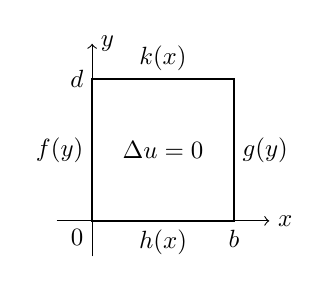
\begin{tikzpicture}[scale=0.9, transform shape]
			\draw [->] (-0.5,0) -- (2.5,0) node[right] {$x$};
			\draw [->] (0,-0.5) -- (0,2.5) node[right] {$y$};
			\draw [thick] (0,0) rectangle (2,2) node[pos=0.5] {$\Delta u = 0$}; 
			\draw (0,0) node[below left] {$0$} (2,0) node[below] {$b$} (0,2) node[left] {$d$};
			\draw (1,0) node[below] {$h(x)$} (0,1) node[left] {$f(y)$} (2,1) node[right] {$g(y)$} (1,2) node[above] {$k(x)$};
		\end{tikzpicture}
	\end{tabular} &
	\begin{tabular}{p{.6\columnwidth}}
		To solve the problem, we divide it into two simpler problems, where $u_1$ is the solution if $h(x) = 0$ and $k(x) = 0$, and $u_2$ if $f(y) = 0$ and $g(y) = 0$. \\
		For this to work, the boundary condition at the corner must be zero, If not, see next section. \\
		Let's solve for Dirichlet and Neumann BC with $k = h = 0$ (in the other case, just flip $x$ and $y$):
	\end{tabular}
\end{tabular}

$$\Delta u = 0 \qquad u(x,y) = X(x) \cdot Y(y) \ \Rightarrow \ \frac{X''(x)}{X(x)} = - \frac{Y''(y)}{Y(y)} = \lambda$$

\begin{tabular}{C{.47\columnwidth}|C{.5\columnwidth}}
	\textbf{Dirichlet}:	$u(0,y) = f, \ u(b,y) = g$ & \textbf{Neumann}: $u_x(0,y) = f, \ u_x(b,y) = g$ \\
	$Y_n(y) = \sin\left(\frac{n\pi}{d} y\right), \ n \in \mathbb{N}$ &
	$Y_n(y) = \cos\left(\frac{n\pi}{d} y\right), \ n \in \mathbb{N}_0 $ \\
\end{tabular}

$$u(x,y) = \sum_n X_n(x) = \sum_n A_n \sinh\left(\frac{n\pi}{d} x\right) + B_n \sinh\left(\frac{n\pi}{d} (x-b)\right)$$

Using this basis ($\sinh$), we have achieved that the term with $A_n$ is zero at $x=0$ and the term $B_n$ is zero at $x = b$. To calculate the constants:

\begin{tabular}{C{.95\columnwidth}}
	\textbf{Dirichlet}:\\
	$\fmm f(x) = u(0,y) = \sum_n B_n \sinh\left(-\frac{n\pi}{d} b\right) \sin\left(\frac{n\pi}{d} y\right) = \sum_n \beta_n \sin\left(\frac{n\pi}{d} y\right)$ \\
	$\fmm g(x) = u(b,y) = \sum_n A_n \sinh\left(+\frac{n\pi}{d} b\right) \sin\left(\frac{n\pi}{d} y\right) = \sum_n \alpha_n \sin\left(\frac{n\pi}{d} y\right)$ \\
	$\fmm \beta_n = \frac{2}{d} \int_{0}^{d} f(y) \sin\left(\frac{n\pi}{d} y\right) dy, \quad \alpha_n = \frac{2}{d} \int_0^b g(y) \sin\left(\frac{n\pi}{d} y\right)dy$ \\ \midrule
	\textbf{Neumann}: \\
	$\fmm f(x) = u_x(0,y) = \sum_n \frac{n\pi}{d} B_n \sinh\left(-\frac{n\pi}{d} b\right) \cos\left(\frac{n\pi}{d} y\right) = \sum_n \beta_n \cos\left(\frac{n\pi}{d} y\right)$ \\
	$\fmm g(x) = u_x(b,y) = \sum_n \frac{n\pi}{d} A_n \sinh\left(+\frac{n\pi}{d} b\right) \cos\left(\frac{n\pi}{d} y\right) = \sum_n \alpha_n \cos\left(\frac{n\pi}{d} y\right)$ \\
	$\fmm \beta_n = \frac{2}{d} \int_{0}^{d} f(y) \cos\left(\frac{n\pi}{d} y\right) dy, \quad \alpha_n = \frac{2}{d} \int_0^b g(y) \cos\left(\frac{n\pi}{d} y\right)dy$ \\ \midrule
	
\end{tabular}

\subsubsection{Discontinuity on the boundary}

If $G:\partial D \rightarrow \mathbb{R}$ is the boundary condition and $G$ is continuous and if we need to separate the problem into two smaller problems, we can get discontinuities. To avoid this, we define a new problem with boundary conditions: $H := G - P$
$$H(x,y) = G(x,y) - P(x,y), \ P(x,y) = \gamma_0 + \gamma_1 x + \gamma_2 y + \gamma_3 xy, \quad \Delta P = 0$$

Now, we choose $\gamma_0, \gamma_1, \gamma_2, \gamma_3$ such that $H(x,y) = 0$ at the vertices of rectangle:
$$\gamma_0 = G(0,0), \ \gamma_1 = G(b,0) - G(0,0), \ \gamma_2 = G(0,d) - G(0,0), $$
$$ \gamma_3 = G(b,d) - G(0,d) - G(b,0) + G(0,0)$$

\subsubsection{Circular Boundary}

If we have a circular boundary with radius $\hat{r}$, we have $u(r,\phi)$ where $x=r \cos \phi$ and $y = r \sin \phi$. We can write the Laplacian as:

$$\Delta u = u_{rr} + \frac1r u_r + \frac{1}{r^2} u_{\phi \phi} = 0, \quad u(r,\phi) = R(r) \cdot \Phi(\phi), \ \Phi(-\pi) = \Phi(\pi)$$
$$\frac{r^2 R''}{R} + \frac{r R'}{R} = -\frac{\Phi''}{\Phi} = \lambda \ \Rightarrow \ \Phi'' = -\lambda \Phi, \quad R'' + \frac{R'}{r} - \frac{\lambda R}{r^2} = 0$$
$$\Phi(\phi) = A \cos(n \phi) + B \sin(n \phi), \ R(r) = r^n, \ n \in \mathbb{N}_0, \ \lambda = n^2$$
$$u(r,\phi) = \frac{A_0}{2} + \sum_{n \in \mathbb{N}} r^n \left(A_n \cos(n\phi) + b_n \sin(n\phi)\right)$$
$$u(\hat r, \phi) = h(\phi) = \frac{A_0}{2} + \sum_{n \in \mathbb{N}} \hat r^n \left(A_n \cos(n\phi) + b_n \sin(n\phi)\right)$$
$$A_n = \frac{1}{\hat r^n \pi} \int_{-\pi}^{\pi} h(\phi) \cos(n\phi) d\phi, \quad B_n = \frac{1}{\hat r^n\pi} \int_{-\pi}^{\pi} h(\phi) \sin(n\phi) d\phi $$

\textbf{Remark}: if the circle does exclude the center, $R(r)$ can be either $R_1$ or $R_2$:
$$R_1 = \begin{case} r^n \\ r^{-n} \end{case} \quad R_2 = \begin{case}1 \\ \ln r \end{case}$$
$$R_n(r) = C_n r^n + D_n r^{-n}, \ \forall n \in \mathbb{N}, \qquad R_0(r) = R_0 + D_0 \ln r$$

\section{General formulas}

\subsection{Ordinary Differential Equation ODE}

\subsubsection{linear first order ODE}

%$$\frac{dx}{dt} = a(t) x + b(t)$$
%$$x(t) = C e^{A(t)} + e^{A(t)} \cdot \int_{0}^{t} e^{-A(\tau)} b(\tau) d\tau \qquad \text{where} \quad A(t) = \int_{0}^{t}a(\tau)d\tau$$
Solve the ODE: $u'(x) + \lambda u(x) = f(x)$.
First, solve for the \textbf{homogeneous} solution: $u_h(x) = A e^{-\lambda x}$.
For the \textbf{particular} solution, use the following ansatz:
\begin{itemize}
	\item If $f(x)$ is a polynomial of degree $n$, then $u_p(x)$ is also a polynomial of degree $n$. 
	\item If $f(x) = b e^{k x}$, then $u_p(x) = B e^{k x}$. 
	\item If $f(x) = b \cos(k x)$ or $f(x) = b \sin(k x)$, then $u_p(x) = B \cos(k x) + C \sin (k x)$ 
\end{itemize}
Finally, the solution to the equation is: $u(x) = u_h(x) + u_p(x)$

\subsubsection{Nonlinear first order ODE}

$$\frac{du}{dx} = f(u) \;\Rightarrow\; \frac{1}{f(u)} du = 1 dx \;\Rightarrow\; \int \frac{1}{f(u)} du = \int 1 dx $$

\subsection{Fourier series}

$$f(x) = a_0 + \sum_{n=1}^{\infty} a_n \cos \frac{n\pi x}{L} + b_n \sin \frac{n\pi x}{L} $$
$$a_n = \frac{2}{L} \int_{0}^{L} f(x) \cos \frac{n \pi x}{L} \qquad b_n = \frac{2}{L} \int_0^L f(x) \sin \frac{n \pi x}{L} \qquad a_0 = \frac{1}{L}$$

\subsection{Trigonometry}
{\small \centering
\begin{tabular}{r<{\hspace{-8pt}}c<{\hspace{-8pt}}l|r<{\hspace{-8pt}}c<{\hspace{-8pt}}l}
	$\sin(2\alpha)$&$ = $&$2 \sin \alpha \cos \alpha$ &
	$\cos(2\alpha)$&$ = $&$\cos^2 \alpha - \sin^2 \alpha$ \\
	$\sin^2 \alpha$&$ = $&$\frac12 \left(1-\cos 2\alpha\right)$ &
	$\cos^2 \alpha$&$ = $&$\frac12 \left(1+\cos 2\alpha\right)$ \\
	$\sin^3 \alpha$&$ = $&$\frac14 \left(3\sin \alpha - \sin 3\alpha\right)$ &
	$\cos^3 \alpha$&$ = $&$\frac14 \left(3\cos \alpha + \cos 3\alpha\right)$ \\
	$\sin(\alpha \pm \beta)$&$ = $&$\sin \alpha \cos \beta \pm \cos \alpha \sin \beta$ & 
	$\cos(\alpha \pm \beta)$&$ = $&$\cos \alpha \cos \beta \mp \sin \alpha \sin \beta$ \\
	$2\sin \alpha \sin \beta$&$=$&$\cos(\alpha-\beta) - \cos(\alpha + \beta)$ &
	$2\cos \alpha \cos \beta$&$=$&$\cos(\alpha-\beta) + \cos(\alpha + \beta)$ \\
	
\end{tabular}
}

\end{twocolumn}

\end{document}
